\documentclass[10pt]{beamer}
 
\usetheme{metropolis} 
\usepackage{appendixnumberbeamer}

\usepackage{booktabs} 
\usepackage[scale=2]{ccicons}
\usepackage{listings}
 
\definecolor{dkgreen}{rgb}{0,0.6,0}
\definecolor{gray}{rgb}{0.5,0.5,0.5} 
\definecolor{mauve}{rgb}{0.58,0,0.82} 

\lstset{frame=tb,
	language=Java,
	aboveskip=3mm,
	belowskip=3mm,
	showstringspaces=false, 
	columns=flexible,
	basicstyle={\small\ttfamily},
	numbers=none,
	numberstyle=\tiny\color{gray},
	keywordstyle=\color{blue},
	commentstyle=\color{dkgreen},
	stringstyle=\color{mauve},
	breaklines=true,
	breakatwhitespace=true,
	tabsize=3
}

\usepackage{pgfplots}
\usepgfplotslibrary{dateplot}

\usepackage{xspace}
\newcommand{\themename}{\textbf{\textsc{metropolis}}\xspace}

\title{Detecting (Absent) App-to-app Authentication on Cross-device
  Short-distance Channels}
\subtitle{ACSAC, December 9-13, 2019 San Juan}
\date{December 13, 2019}
\author{Stefano Cristalli, Danilo Bruschi, Long Lu, Andrea Lanzi}
\institute{University of Milan Italy, Northeastern University Boston US}
\titlegraphic{\hfill
  
\includegraphics[height=1.5cm]{unimi.png}
   
\includegraphics[height=1.5cm]{ne2.png}
 }
  

\begin{document}

\maketitle 

\begin{frame}{Outline}
  \setbeamertemplate{section in toc}[sections numbered]
  \tableofcontents[hideallsubsections]
\end{frame}

\section{Introduction}
\begin{frame}[fragile]{Context}
  \begin{itemize}

  \item Cross-device communications allow nearby devices to directly
    communicate bypassing cellular base stations (BSs) or access
    points (APs) (e.g. {\bf spectral efficiency improvement, energy
      saving, and delay reduction}, etc.)

  \item Without the need for infrastructure, {\bf such a technology
      enables mobile users (e.g., Android) to instantly share
      information (e.g., pictures and videos)}

  \item Such technology is also predominat in {\bf IoT environment}
    where a mobile device is direct connected to the embedded system.

  \end{itemize}

 \end{frame}




 
\begin{frame}[fragile]{Cross-device Authentication Scheme}

  %\begin{itemize}

  %\item Currently, most cross-device, peer-to-peer communications
  %  channels are authenticated by using an {\bf out-of-band scheme}.

  %\end{itemize}
   
  \begin{figure}[bhp]
    \centering
	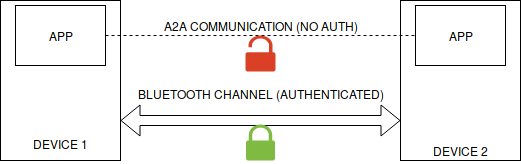
\includegraphics[width=80mm]{img/2-background}
     \end{figure}

     \begin{figure}[bhp]
    \centering
	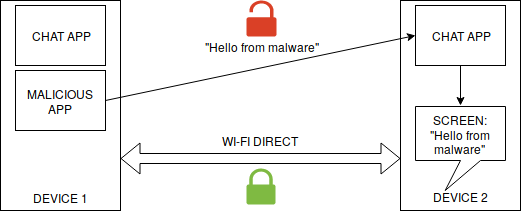
\includegraphics[width=80mm]{img/2-malware}
     \end{figure}
  
 
  
\end{frame}

\begin{frame}[fragile]{Threat Model \& Attack}

  \begin{itemize}


  \item The attacker is able to install a malicious app on the
    mobile's victim phone.

  \item The malicious app can therefore craft custom messages to send
    to the other device, which are displayed as if they were sent from
    the original app.

  \item Depending on the particular context, there are some scenarios
    in which the attack can become very dangerous: {\bf Phishing,
      Malware delivery, Exploitation}.

  \end{itemize}

  
\end{frame}

\begin{frame}[fragile]{Current Solutions}
  \begin{itemize}

  \item Several solutions exist for securing cross-device
    communication.  In the Android environment, they allow
    {\bf authentication of devices and communication channels}.

  \item Others solutions {\bf restricts apps’ access to external
      resources, such as Bluetooth, SMS and NFC}, by defining new
    SEAndroid types to represent the resources.

  \item Moroever such {\bf solutions are not able to address several
      communication channels such as: SMS, Audio, Wi-Fi and NFC} due
    to of missing important information for the detection purpose.

  \end{itemize} 

  
\end{frame}


\begin{frame}[fragile]{Contributions}


 \begin{itemize}
  
 %\item This problem is due to the fact that the authentication between
 %  apps is missing. {\bf We name this security issue cross-device
 %    app-to-app communication hijacking, or CATCH}.

 \item We identify a security problem called {\bf cross-device
     app-to-app communication hijacking (CATCH)}, which commonly
   exists in Android apps that use short-distance channels, and
   afflicts all the tested Android version.

 \item We provide a solution to the CATCH problem by {\bf designing
     and developing an authentication scheme detector} that analyzes
   Android apps to discover potential vulnerabilities

% \item {\bf Validate the results of our system on Android apps} with
%   manual analysis, and test its resilience in detecting the
%   authentication scheme.

\end{itemize}
  
\end{frame}



\section{CATCH Detection}

\begin{frame}[fragile]{Authentication Scheme Definitions}

  \begin{itemize}

  \item Such form of authentication proposes authenticated information
    exchange between devices. {\bf These are called out-of-band,
      side-channels or location-limited channels (LLCs).}

  \item Then the apps can share a secret and they can start sending
    data, {\bf using the secret as authenticator}, appending the
    secret as a form of nounce to protect the messagge.

  \item When the messagge has been received the app needs to perform
    authentication checks. {\bf These checks must occur before any
      critical use of the data, otherwise the communication is not
      authenticated.}
      
  \end{itemize}

  
\end{frame}


\begin{frame}[fragile]{Challenges}

  \begin{itemize}

  \item We need to define a {\bf generic scheme that captures the es-
      sential logic of app-to-app authentication}.

  \item We need to define a strategy for differentiating between an
    if-statement that does not operate on security critical data and
    an {\bf if-statement that is a part of the authentication scheme}.

  \item Additionally, the authentication scheme {\bf can be
      implemented in several ways according to the developer
      experience}. This adds an additional layer of difficulty for our
      analysis (e.g., obfuscation).

  \end{itemize}
  
\end{frame}


\begin{frame}[fragile]{Detection Strategy}

  We define two main check points for our algorithm:
  \begin{itemize}

  \item An {\bf entry point} is an instruction in the code that
      indicates the start of the communication over the analyzed
      channel (e.g., data receiving)

    \item An {\bf exit point} is represented by the first
      authenticated use of the data coming from the monitored channel.

   \end{itemize}
  
\end{frame}

\begin{frame}[fragile]{Detection Algorithm}

 \begin{figure}[bhp]
    \centering
	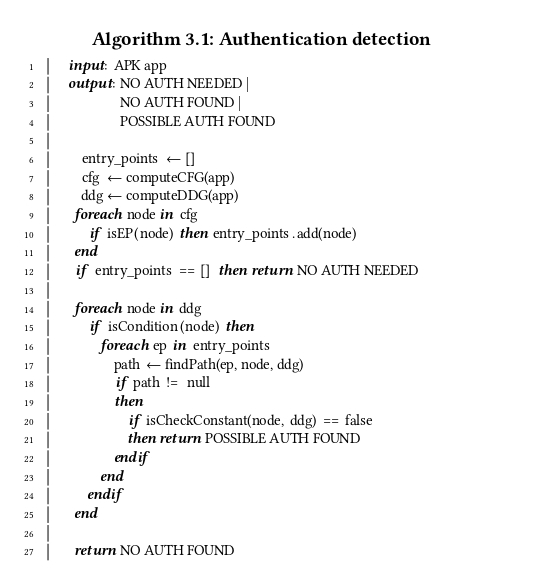
\includegraphics[width=65mm]{img/algo}
     \end{figure}
  
\end{frame}

\begin{frame}[fragile]{Reducing False Positive}

  \begin{itemize}

  \item In our context, the analyzed authentication model must be
    performed with some sort of {\bf dynamically generated secret}
    that is usually stored in the dynamic memory (e.g., heap, stack).

  \item By using {\bf constant propagation} we can discard all the
    conditions that use constant values in their comparison, and {\bf
      we only consider comparison between the input and dynamic
      values.}

  \item Constant propagation is a very powerful technique for our
    analysis, and it helps to reduce the false positives to 0\%


  \end{itemize}
  
\end{frame}



%\section{Technical Details}
%\begin{frame}[fragile]{Technical Details} 

%\begin{itemize}

%\item Our system is composed of three main components: (1) {\bf Graphs
%  Builder}, (2) {\bf Path Finder} and (3) {\bf App-to-app Authentication
%  Finder} and it is based on ARGUS-SAF. 

%\item (1) builds an inter-component control flow graph {\bf (ICFG)}
%  and intercomponent data flow graph of the whole app. Finally, the
%  framework builds a data dependency graph (DDG) on top the {\bf
%    IDFG}.

%\item (2) The Path Finder component traverses the CFG received from
%  Graphs Builder, and {\bf marks entry points for the analyzed channel}
%  based on a predefined list of method signatures.
 
%\item (3) App-to-app Authentication Finder applies {\bf further
%    checks} to the paths received from Path Finder, in order {\bf to
%    exclude false positive} results by recognizing checks against
%  constant values.
 

%\end{itemize}
%\end{frame}

\section{Experimental Evaluation}
\begin{frame}[fragile]{Experimental Evaluation}

  To test our system we divided the experiments into two main categories:
  \begin{itemize}

  \item {\bf A dataset analysis on APKs retrieved from a research
    repository}, aiming at confirming the efficacy of the
    algorithm on negative samples;

  \item {\bf A targeted analysis on custom apps} built by applying
    code transformation techniques (e.g. obfuscation) for proving that
    the authentication scheme is correctly detected by our algorithm.
      
  \end{itemize}
	
\end{frame}

\begin{frame}[fragile]{Dataset Composition}
 
  \begin{itemize}

  \item We ran tests on a large number of APKs collected from the
    {\bf Androzoo repository}, crawled from {\bf several Android markets:
      Google Play, Anzhi and AppChina}.

  \item We started analyzing a total of {\bf 210,425 APKs}, randomly
    chosen from the Androzoo repository. In order to select the
    appropriate Bluetooth APKs we applied the {\bf Bluetooth filter}
    and we obtained a total of {\bf 2,739 APKs}.
 
  \item We discovered that 704 of the selected apps do not have any
    entry point for Bluetooth communication in the CFG. we obtained a
    number of {\bf 238 APKs, suitable for our analysis and
      evaluation}.

    \item Obfuscation filter selected a total of {\bf 942 APKs from the
      initial set of 2,793}, which means that the majority of the apps
    in our dataset, almost {\bf 70\%, use ProGuard for code
      obfuscation}.

    


  \end{itemize}

  
\end{frame}

\begin{frame}[fragile]{Dataset Composition}

  We analyzed the composition of our dataset to make sure that we did
  not run tests on sample/unused/abandoned apps.
  
  \begin{itemize}
    
  \item We sampled 200 APKs (containing permissions/classes for
    Bluetooth) from our dataset, and performed a manual analysis by
    searching them on Google Play.
    \begin{itemize}

    \item {\bf Game apps}, where Bluetooth is used for playing peer-to-peer

    \item {\bf IoT apps for specific devices}, where Bluetooth is used
      to send and receive data from the controlled device or sensors

    \item {\bf Business/health apps}, using Bluetooth to send data
      from smartphone to computer, or again smartphone to device
    
  \end{itemize}

  \end{itemize}
  
\end{frame}



\begin{frame}[fragile]{Results}

\begin{itemize}

\item We run our algorithm on {\bf 238 Apps without constant
    propagation} we obtained {\bf 11\% of false positive}. With
  constant propagation enable we reach {\bf 0\% of false positive}.

\item We built a custom app using Bluetooth that use out-of-band
  authentication and we applied Proguard transformation on the
  app. {\bf We found that our algorithm correctly predicts the
    possible presence of authentication}

\item We decided to run our tool on ProGuard-obfuscated APKs from our
  dataset a total of 662 APKs. {\bf 100\% of the APKs were identified
    as negative (i.e., not containing authentication) by our tool.}
  

\end{itemize}

\end{frame}

\begin{frame}[fragile]{Performance Analysis}

  To set up a correct time threshold we need to be sure that the
  constructed CFG and DDG include the Bluetooth entry points and the
  authentication checks. we set up three Threshold 30, 60, 120 sec.
  
\begin{itemize}

\item For any entry point, we found on average more than {\bf 10,000
    instructions that are dominated by the entry point and the CFG
    reachability from a single entry point to any node in the graph}.
  
\item The {\bf variation of the results between the three runs is
    minimal}, that it means that we generally do not miss any
  important information.
  
\item The average time spent for {\bf modeling the APK in Argus-SAF is
    5 minutes}, while the {\bf average running time of our algorithm}
  on the generated graphs is {\bf 2 minutes}, giving a total average
  {\bf time of 7 minutes}.
  
\end{itemize}

\end{frame}


\section{Case Studies}
\begin{frame}[fragile]{Data injection on BluetoothChat and Wifi-Direct}

  \begin{itemize}

  \item We implement the attack vector against two real applications:
    (1) {\bf BluetoothChat} that use Bluetooth technology, (2) {\bf
      Filesharing} on Wi-Fi Direct.

  \item Two preliminaries requirements: (1) the malicious app needs to
    recognize the {\bf presence of the target application}. (2) the
    malicious app needs to detect when the target {\bf application is
      opened and run.}

  \item If the attacker has satisfied the previous two requirements
    the attack can be performed successfully.

  \end{itemize}
  
  
\end{frame}


\section{Limitations}
\begin{frame}[fragile]{Impact \& Limitations}

\begin{itemize}

\item Our framework is not able to handle particular intra-component
  and inter-component transitions, such as ones performed with {\bf
    reflection}, and it cannot correctly {\bf model concurrency}.

\item In case of authentication, we {\bf expect to see controls on
    data read from the channel immediately after a read operation},
  following our authentication model.

\item We manually analyzed {\bf 20 Android apps from 662 dataset apps}
  and we check whether threads functions defined in the apps include
  any authentication scheme ({\bf false negative results}).

\end{itemize}

\end{frame}

\section{Conclusion}
\begin{frame}[fragile]{Conclusion}
  
  \begin{itemize}
    
  \item We have shown the extension and potential impact of {\bf CATCH
      vulnerabilities in Android apps}, providing a threat model and
    specific definitions for the problem,

  \item {\bf We design an automated system for APK analysis}, is a
    first line of defense against human error, and could be used to
    identify vulnerable apps.

  \item {\bf We test the efficacy and efficiency of our system}
    against a large number of android apps.
  
\end{itemize}
\end{frame}

\section*{Thank you for attention}

\section*{Questions?}

\end{document}
